% =====================================================================
%  ACL-style paper distilled from the bachelor's thesis
%  "When Does Memory Help an LLM Judge?"
%  Khush Patel, Bader Rasheed, Innopolis University, 2026
% =====================================================================
\documentclass[11pt]{article}
\usepackage[final]{acl}
\usepackage{times}
\usepackage{latexsym}
\usepackage[T1]{fontenc}
\usepackage[utf8]{inputenc}
\usepackage{microtype}
\renewcommand{\ttdefault}{lmtt}
\usepackage{graphicx}
\usepackage{booktabs}
\usepackage{amsmath}
\usepackage{amssymb}
\usepackage{amsthm}
\usepackage{tikz}
\usetikzlibrary{positioning, arrows.meta}
\newtheorem{proposition}{Proposition}

\title{When Does Memory Help an LLM Judge? \\ A Provably Leakage-Free, Audited Evaluation of Memory-Augmented Judging}


\author{draft \\
  Innopolis University \\
  \texttt{@innopolis.university} }


% \author{Khush Patel \\
%   Innopolis University \\
%   \texttt{k.patel@innopolis.university} \\\And
%   Bader Rasheed \\
%   Innopolis University \\
%   \texttt{b.rasheed@innopolis.university} \\}



\begin{document}
\maketitle

\begin{abstract}
Giving an LLM judge a persistent memory of its past evaluations seems like it should help. We build such a judge and evaluate it under two protocols. Under a conventional protocol (memory updated during evaluation, related test items not separated), memory appears to add 6--10 accuracy points; under a careful one, the gain disappears. The careful protocol is leakage-free (question-level data split plus frozen memory) with a two-layer audit (SHA-256 graph fingerprints plus runtime write-blocking) that proves, for every run, that memory was not modified during evaluation. Under this protocol, with GPT-4o, no memory or tree-search configuration significantly outperforms a plain stateless judge, and an apparent catastrophic collapse under memory poisoning turns out to be a harness defect, not a system property. A per-item verdict analysis explains the null: memory changes only 10\% of verdicts, and the verdicts it changes follow the judge's leniency bias rather than the ground truth. We bound the achievable benefit of memory by the conditional information it carries about the label plus the judge's own decision noise, characterize when memory should help, and propose practical remedies. The protocol and audit are released as a reusable instrument.
\end{abstract}

\section{Introduction}

LLMs now grade other LLMs. A judge model reads a task, a candidate response, and a rubric, and returns a verdict \citep{mt_bench2023, geval2023, judge_survey2024}; these verdicts rank chatbots, score agents, and feed reward signals during training, so whether the judge can be trusted matters \citep{chateval2023, llm_judge_agreement2024}.

A standard judge is stateless. It sees each item in isolation, so it cannot recognize a near-identical past case, reuse a good line of reasoning, or learn from a mistake. A natural remedy is memory: let the judge retrieve its relevant past evaluations before deciding, in the spirit of retrieval-augmented generation \citep{rag_original2020} and agent memory systems \citep{memgpt2023, generative_agents2023, reflexion2023}.

We built exactly this system. The complication is that memory is also a leakage channel. A store of past evaluations can propagate old errors, can be poisoned \citep{rag_poisoning2024}, and, most subtly, can carry information about a test item into the evaluation of that same item. Contamination is a known way to inflate benchmark scores \citep{data_contamination2024, benchmark_contamination2024, eval_leakage2024}, and a memory written during evaluation is a direct contamination channel. Prior memory-augmented systems assume this is not happening; none verifies it.

We verify it. The contributions:

\begin{enumerate}
    \item \textbf{A protocol that proves the absence of leakage instead of assuming it} (\S\ref{sec:protocol}): split the benchmark by question so paired pass/fail items never straddle the split, freeze memory during evaluation, and verify the freeze with a two-layer audit (a SHA-256 fingerprint of the entire memory graph taken before and after evaluation, plus runtime interception of every write). The audit is mechanical: a hash either matches or it does not.
    \item \textbf{A corrective null result} (\S\ref{sec:results}). Under the audited protocol, none of our memory or tree-search configurations significantly beats the stateless GPT-4o judge: not with the judge's own memory, not with oracle (ground-truth) memory, not with a simpler schema, not on other random seeds. The audit also caught a real write-back leakage bug in our own evaluation path on its first run, and a corrected harness showed that an apparent collapse to 21.2\% accuracy under 50\% memory poisoning was caused by network errors being scored as wrong answers.
    \item \textbf{An explanation, not just a number} (\S\ref{sec:analysis}). We read the per-item verdicts instead of stopping at aggregate accuracy. Memory leaves 90\% of verdicts unchanged, and the verdicts it does change flip mostly toward ``pass'' and are mostly wrong: memory acts as a leniency anchor that amplifies the judge's existing class bias instead of contributing evidence. We formalize this with a Bayes-ceiling argument: memory can raise the achievable accuracy only insofar as the conditional label distribution $P(Y\mid X,M)$ differs from $P(Y\mid X)$, which the leakage-free protocol drives to near-equality, while the separate channel of stabilizing the realized (stochastic) judge has at most the judge's measured 5--10\% self-disagreement to work with. The same account predicts when memory \emph{should} help and yields concrete fixes: balanced contrastive retrieval, similarity-gated injection, and population-level calibration.
\end{enumerate}

\section{Related Work}

\paragraph{LLM-as-a-Judge.} G-Eval, MT-Bench, and Prometheus \citep{geval2023, mt_bench2023, prometheus2023} showed LLM judges can track human raters. The judges also carry position, length, and self-preference biases \citep{llm_judge_bias2024, position_bias2024}, fragile agreement, and poor calibration \citep{chateval2023, llm_judge_agreement2024, judge_calibration2024}. A stateless judge additionally has no way to be consistent across related items, which is the opening for memory.

\paragraph{Retrieval- and memory-augmented systems.} RAG \citep{rag_original2020} and its adaptive variants \citep{active_rag2023, self_rag2023} condition generation on retrieved evidence. Agent memory systems such as MemGPT \citep{memgpt2023}, Generative Agents \citep{generative_agents2023}, and Reflexion \citep{reflexion2023} store episodes or self-feedback for reuse. A memory-augmented judge retrieves past evaluations as contrastive references. None of this prior work treats memory as a leakage source or organizes it as a typed graph.

\paragraph{Test-time search.} Chain-of-Thought \citep{chain_of_thought2022}, Self-Consistency \citep{self_consistency2023}, Tree of Thoughts \citep{tree_of_thoughts2023}, and ReAct \citep{react2023} spend more inference compute for better reasoning; MCTS-Judge \citep{mcts_judge2025} applies Monte Carlo Tree Search \citep{uct2006, mcts_survey2012} to judging. Our MCTS components follow this line; under the audited protocol they cost $9\times$ the latency with no significant gain, and we report them as exploratory.

\paragraph{Contamination and leakage.} Contamination inflates scores \citep{data_contamination2024, benchmark_contamination2024, eval_leakage2024}, and PoisonedRAG \citep{rag_poisoning2024} corrupts outputs through small injections into a retrieval store. We name the two channels specific to memory-augmented judging, paired-item leakage and write-back leakage, and close both provably.

\section{The Memory-Augmented Judge}
\label{sec:system}

\paragraph{Typed memory graph.} Memory lives in a Neo4j property graph \citep{neo4j2023} with five node types: \textbf{Policy} (a grading rule), \textbf{Attempt} (a past response with its verdict and reasoning), \textbf{Issue} (a specific problem found), \textbf{Fix} (a correction), and \textbf{Semantic} (a category grouping similar issues), linked by four typed relations (Figure~\ref{fig:schema}). Every node carries a 1536-dimensional embedding \citep{openai_embeddings2024} under an HNSW index \citep{hnsw2018}.

\begin{figure}[t]
\centering
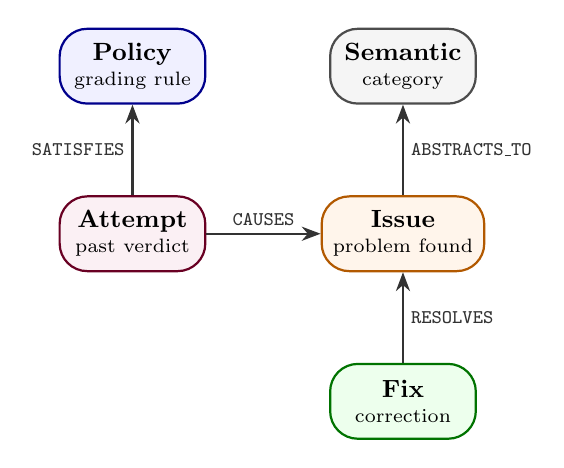
\begin{tikzpicture}[
  font=\small,
  gnode/.style={draw, rounded corners=10pt, align=center, inner sep=4pt,
                minimum height=0.95cm, minimum width=1.85cm, thick},
  rel/.style={-{Stealth[length=2.4mm]}, thick, gray!40!black},
  rlab/.style={font=\scriptsize\ttfamily, fill=white, inner sep=1.5pt}
]
\node[gnode, draw=blue!55!black,   fill=blue!6]
  (policy)  {\textbf{Policy}\\[-2pt]{\scriptsize grading rule}};
\node[gnode, draw=purple!55!black, fill=purple!6, below=1.15cm of policy]
  (attempt) {\textbf{Attempt}\\[-2pt]{\scriptsize past verdict}};
\node[gnode, draw=orange!70!black, fill=orange!8, right=1.45cm of attempt]
  (issue)   {\textbf{Issue}\\[-2pt]{\scriptsize problem found}};
\node[gnode, draw=gray!60!black,   fill=gray!8, above=1.15cm of issue]
  (semantic){\textbf{Semantic}\\[-2pt]{\scriptsize category}};
\node[gnode, draw=green!45!black,  fill=green!7, below=1.15cm of issue]
  (fix)     {\textbf{Fix}\\[-2pt]{\scriptsize correction}};
\draw[rel] (attempt) -- node[rlab, left=1pt]  {SATISFIES}     (policy);
\draw[rel] (attempt) -- node[rlab, above=1pt] {CAUSES}        (issue);
\draw[rel] (fix)     -- node[rlab, right=1pt] {RESOLVES}      (issue);
\draw[rel] (issue)   -- node[rlab, right=1pt] {ABSTRACTS\_TO} (semantic);
\end{tikzpicture}
\caption{The typed memory graph. Each judged item produces an Attempt linked to its Policy; extracted Issues, their Fixes, and abstract Semantic categories structure the judge's past experience. Every node carries a text embedding for similarity retrieval.}
\label{fig:schema}
\end{figure}

\paragraph{Memory-assisted judge (MAJ).} A single-pass judge whose prompt is conditioned on three retrieval stages: (i) similar past attempts, split into passing and failing sets for a contrastive signal; (ii) similar past issues; (iii) recurring issue categories. The similarity thresholds are asymmetric (positive $\ge 0.85$, negative $\ge 0.92$); they were set heuristically during development, and \S\ref{sec:analysis} shows the asymmetry has a measurable consequence.

\paragraph{Exploratory MCTS components.} \emph{MCTS-Judge} decomposes one evaluation into 5--7 generated subtasks and searches over reasoning trajectories with UCT plus an LLM self-assessment. \emph{MCTS-Retrieval} replaces the fixed pipeline with tree search over seven graph retrieval actions, four of them multi-hop. Crossing memory and search gives the ablation modes: \emph{Stateless}, \emph{MAJ}, \emph{MCTS-Judge}, and \emph{MCTS-Judge+Memory}.

\section{Leakage-Free Protocol and the Frozen-Memory Audit}
\label{sec:protocol}

\subsection{Two leakage channels}

The benchmark (\S\ref{sec:setup}) is paired: every question appears twice, once with a passing response and once with a failing one. That pairing creates two accidental leakage paths. \textbf{Paired-item leakage}: split the data by row and one version of a question can land in memory while its twin lands in the test set; when the judge retrieves the twin, it is effectively shown the answer. \textbf{Write-back leakage}: update memory during testing and the verdict on an early item becomes retrievable while scoring a later, related one. Either channel inflates accuracy with zero improvement in judging.

\subsection{Protocol}

Two rules. \textbf{Split by question, not by row}: unique questions are shuffled with a fixed seed and divided in half, and both versions of a question stay on the same side. \textbf{Freeze memory}: memory is built once, before evaluation, and is read-only during the test.

\subsection{The two-layer audit}

A stated freeze is a claim, not a proof. We require the proof, per run (Figure~\ref{fig:audit}).

\begin{figure}[t]
\centering
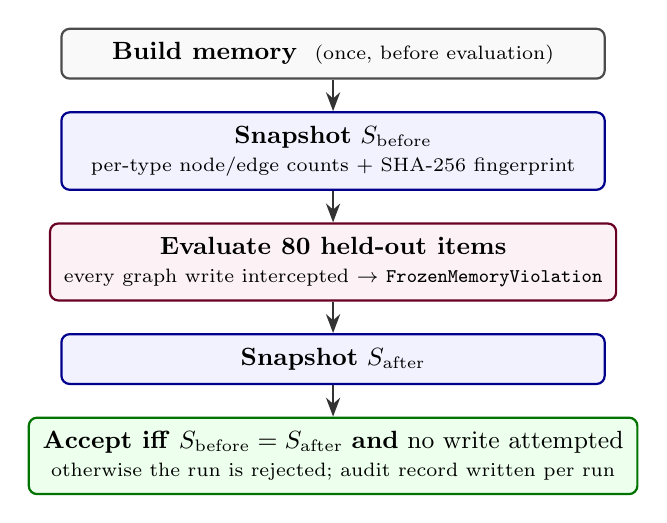
\begin{tikzpicture}[
  font=\small,
  astep/.style={draw, rounded corners=3pt, align=center, inner sep=5pt,
               minimum width=6.9cm, thick},
  rel/.style={-{Stealth[length=2.4mm]}, thick, gray!40!black},
  node distance=0.4cm
]
\node[astep, draw=gray!60!black, fill=gray!5] (build)
  {\textbf{Build memory} \ {\scriptsize(once, before evaluation)}};
\node[astep, draw=blue!55!black, fill=blue!5, below=of build] (before)
  {\textbf{Snapshot} $S_{\text{before}}$\\[-1pt]
   {\scriptsize per-type node/edge counts + SHA-256 fingerprint}};
\node[astep, draw=purple!55!black, fill=purple!5, below=of before] (eval)
  {\textbf{Evaluate 80 held-out items}\\[-1pt]
   {\scriptsize every graph write intercepted $\rightarrow$ \texttt{FrozenMemoryViolation}}};
\node[astep, draw=blue!55!black, fill=blue!5, below=of eval] (after)
  {\textbf{Snapshot} $S_{\text{after}}$};
\node[astep, draw=green!45!black, fill=green!7, below=of after] (verdict)
  {\textbf{Accept iff} $S_{\text{before}} = S_{\text{after}}$ \textbf{and} no write attempted\\[-1pt]
   {\scriptsize otherwise the run is rejected; audit record written per run}};
\draw[rel] (build)  -- (before);
\draw[rel] (before) -- (eval);
\draw[rel] (eval)   -- (after);
\draw[rel] (after)  -- (verdict);
\end{tikzpicture}
\caption{The two-layer frozen-memory audit. Layer 1 (snapshots) detects any mutation after the fact; layer 2 (write interception) prevents it during the run. A run is accepted only if both layers pass.}
\label{fig:audit}
\end{figure}

\textbf{Layer 1, after the fact:} immediately before and after evaluation, take a deterministic snapshot of the graph (per-type node and edge counts, plus a SHA-256 fingerprint over the sorted node identifiers and edge triples). Accept the run only if the counts and fingerprints match exactly. The before/after record is written to a per-run audit file.

\textbf{Layer 2, during the run:} patch every write method of the graph interface with a guard that raises \texttt{FrozenMemoryViolation} if called. A code path that tries to write during evaluation dies loudly instead of corrupting the run silently.

\textbf{The audit was not a formality.} On its first application to MCTS-Judge+Memory it failed: the graph grew from 412 to 492 nodes and 831 to 1003 edges, because our own evaluation path was writing each just-judged test item back into memory. That is exactly the write-back leakage the protocol exists to prevent, found in our own code. We fixed it with a read-only evaluation mode; every number below has a passing audit record. Note the audit cannot be steered toward a desired outcome: its verdict is a hash comparison and an exception, it was built before the audited results were generated, and its first action was to fail on our own code.

\subsection{Memory provenance conditions}

Four conditions isolate where memory comes from and how good it is: \textbf{no-memory} (empty graph); \textbf{self-written} (the judge's own verdicts, reasoning, issues, and fixes from the memory-building half; this is how memory grows in deployment, errors included); \textbf{oracle} (ground-truth labels stored directly, guaranteed correct); and \textbf{poisoned} (oracle memory with a deterministic 10/20/50\% of labels flipped).

\section{Experimental Setup}
\label{sec:setup}

\paragraph{Dataset.} EvalsBench \citep{evalsbench2024} is an open benchmark (Apache-2.0) of 160 graded question--answer pairs over 80 unique questions in the startup and financial-analysis domain. Each row has a topic, question, grading rubric, candidate response, and a balanced pass/fail target (80/80). Each question appears exactly twice, with one passing and one failing response, which makes the benchmark a natural stress test for paired-item leakage. Under the protocol, 40 questions (80 samples) build memory and 40 questions (80 samples) are the held-out test set, seed 42 unless stated.

\paragraph{Judge and search budget.} The judge is GPT-4o, pinned to a fixed API version; all per-sample inputs, verdicts, and audit records are released,\footnote{\url{https://github.com/khushpatel2002/MCTS-MAJ}} so every statistic is re-derivable without re-querying the model. MCTS modes use two rollouts at maximum depth three; a sweep to four rollouts and depth five changed nothing at $4\times$ the cost. All decision extraction uses schema-validated structured outputs \citep{pydantic2024}; an earlier regex extractor failed silently on 15--20\% of responses, a failure mode that can silently masquerade as an empirical finding.

\paragraph{Statistics.} Every accuracy carries a two-sided Wilson 95\% CI \citep{wilson1927}. Mode comparisons are paired on identical items, with the exact McNemar test \citep{mcnemar1947} and a paired bootstrap 95\% CI (10{,}000 resamples) \citep{bootstrap1993}; we call a difference significant only if $p<0.05$ \emph{and} the bootstrap interval excludes zero. This joint rule is conservative with respect to multiple comparisons; we apply no further correction because every primary comparison already fails to reject, and a correction only strengthens that conclusion. Observed effects are also small on a standardized scale (Cohen's $h \approx 0.1$ for the largest clean-memory delta). Samples that still fail after exponential-backoff retries are recorded with a null verdict and excluded, with the completed $n$ reported. This detail is material: \S\ref{sec:poisoning} shows it is the difference between the true result and a spurious headline finding.

\section{Results}
\label{sec:results}

\subsection{The motivating observation}

Before the protocol existed, we measured the system conventionally: memory updated during evaluation, paired questions not separated. Memory appeared to help substantially: gains of 6--10 points across capable judge models, and seeding memory with ground-truth examples appeared to lift cold-start accuracy from 78\% to 91\%. We did not retain per-sample logs for these runs, so we report them only as the motivating observation. Several of these configurations contain one or both leakage channels by construction, which is precisely the methodological problem this paper addresses.

\subsection{Clean-memory comparison}

\begin{table}[t]
\centering
\small
\begin{tabular}{lccc}
\toprule
Mode & Acc.\ [95\% CI] & $n$ & Lat. \\
\midrule
Stateless & 70.0 [59.2, 78.9] & 80 & 3.6\,s \\
MAJ (self-written) & 65.0 [54.1, 74.5] & 80 & 4.5\,s \\
MCTS-Judge & 70.0 [59.2, 78.9] & 80 & 31.8\,s \\
MCTS-J.+Mem. & 71.8 [61.0, 80.6] & 78 & 33.3\,s \\
\bottomrule
\end{tabular}
\caption{Clean-memory results under the leakage-free, audited protocol (GPT-4o, held-out $n{=}80$).}
\label{tab:clean}
\end{table}

Table~\ref{tab:clean} shows the central result: no configuration outperforms the stateless baseline. MAJ vs.\ stateless is $-5.0$ points (bootstrap CI $[-12.5, +1.3]$, McNemar $p{=}0.29$); MCTS-Judge vs.\ stateless is exactly $0.0$; MCTS-Judge+Memory vs.\ stateless is $+1.8$ ($p{=}0.80$). Every confidence interval overlaps the baseline (Figure~\ref{fig:accuracy}); every paired difference crosses zero (Figure~\ref{fig:deltas}). The 6--10 point gain from the conventional protocol is gone. We changed the measurement, not the system.

\begin{figure}[t]
\centering
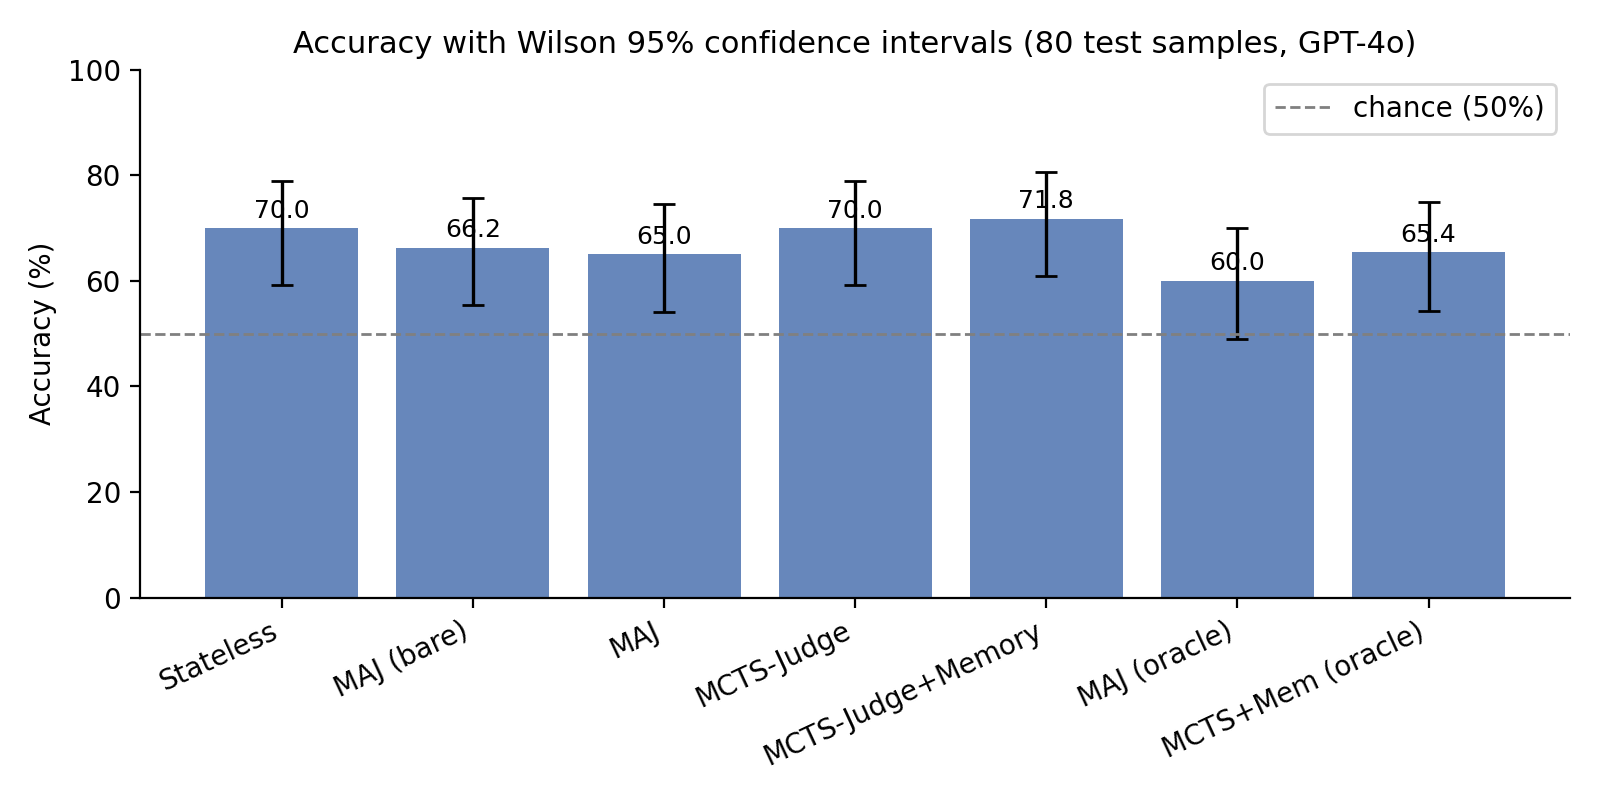
\includegraphics[width=\columnwidth]{figures/accuracy_ci.png}
\caption{Per-mode accuracy with Wilson 95\% CIs on the audited test set; every interval overlaps the stateless baseline.}
\label{fig:accuracy}
\end{figure}

\begin{figure}[t]
\centering
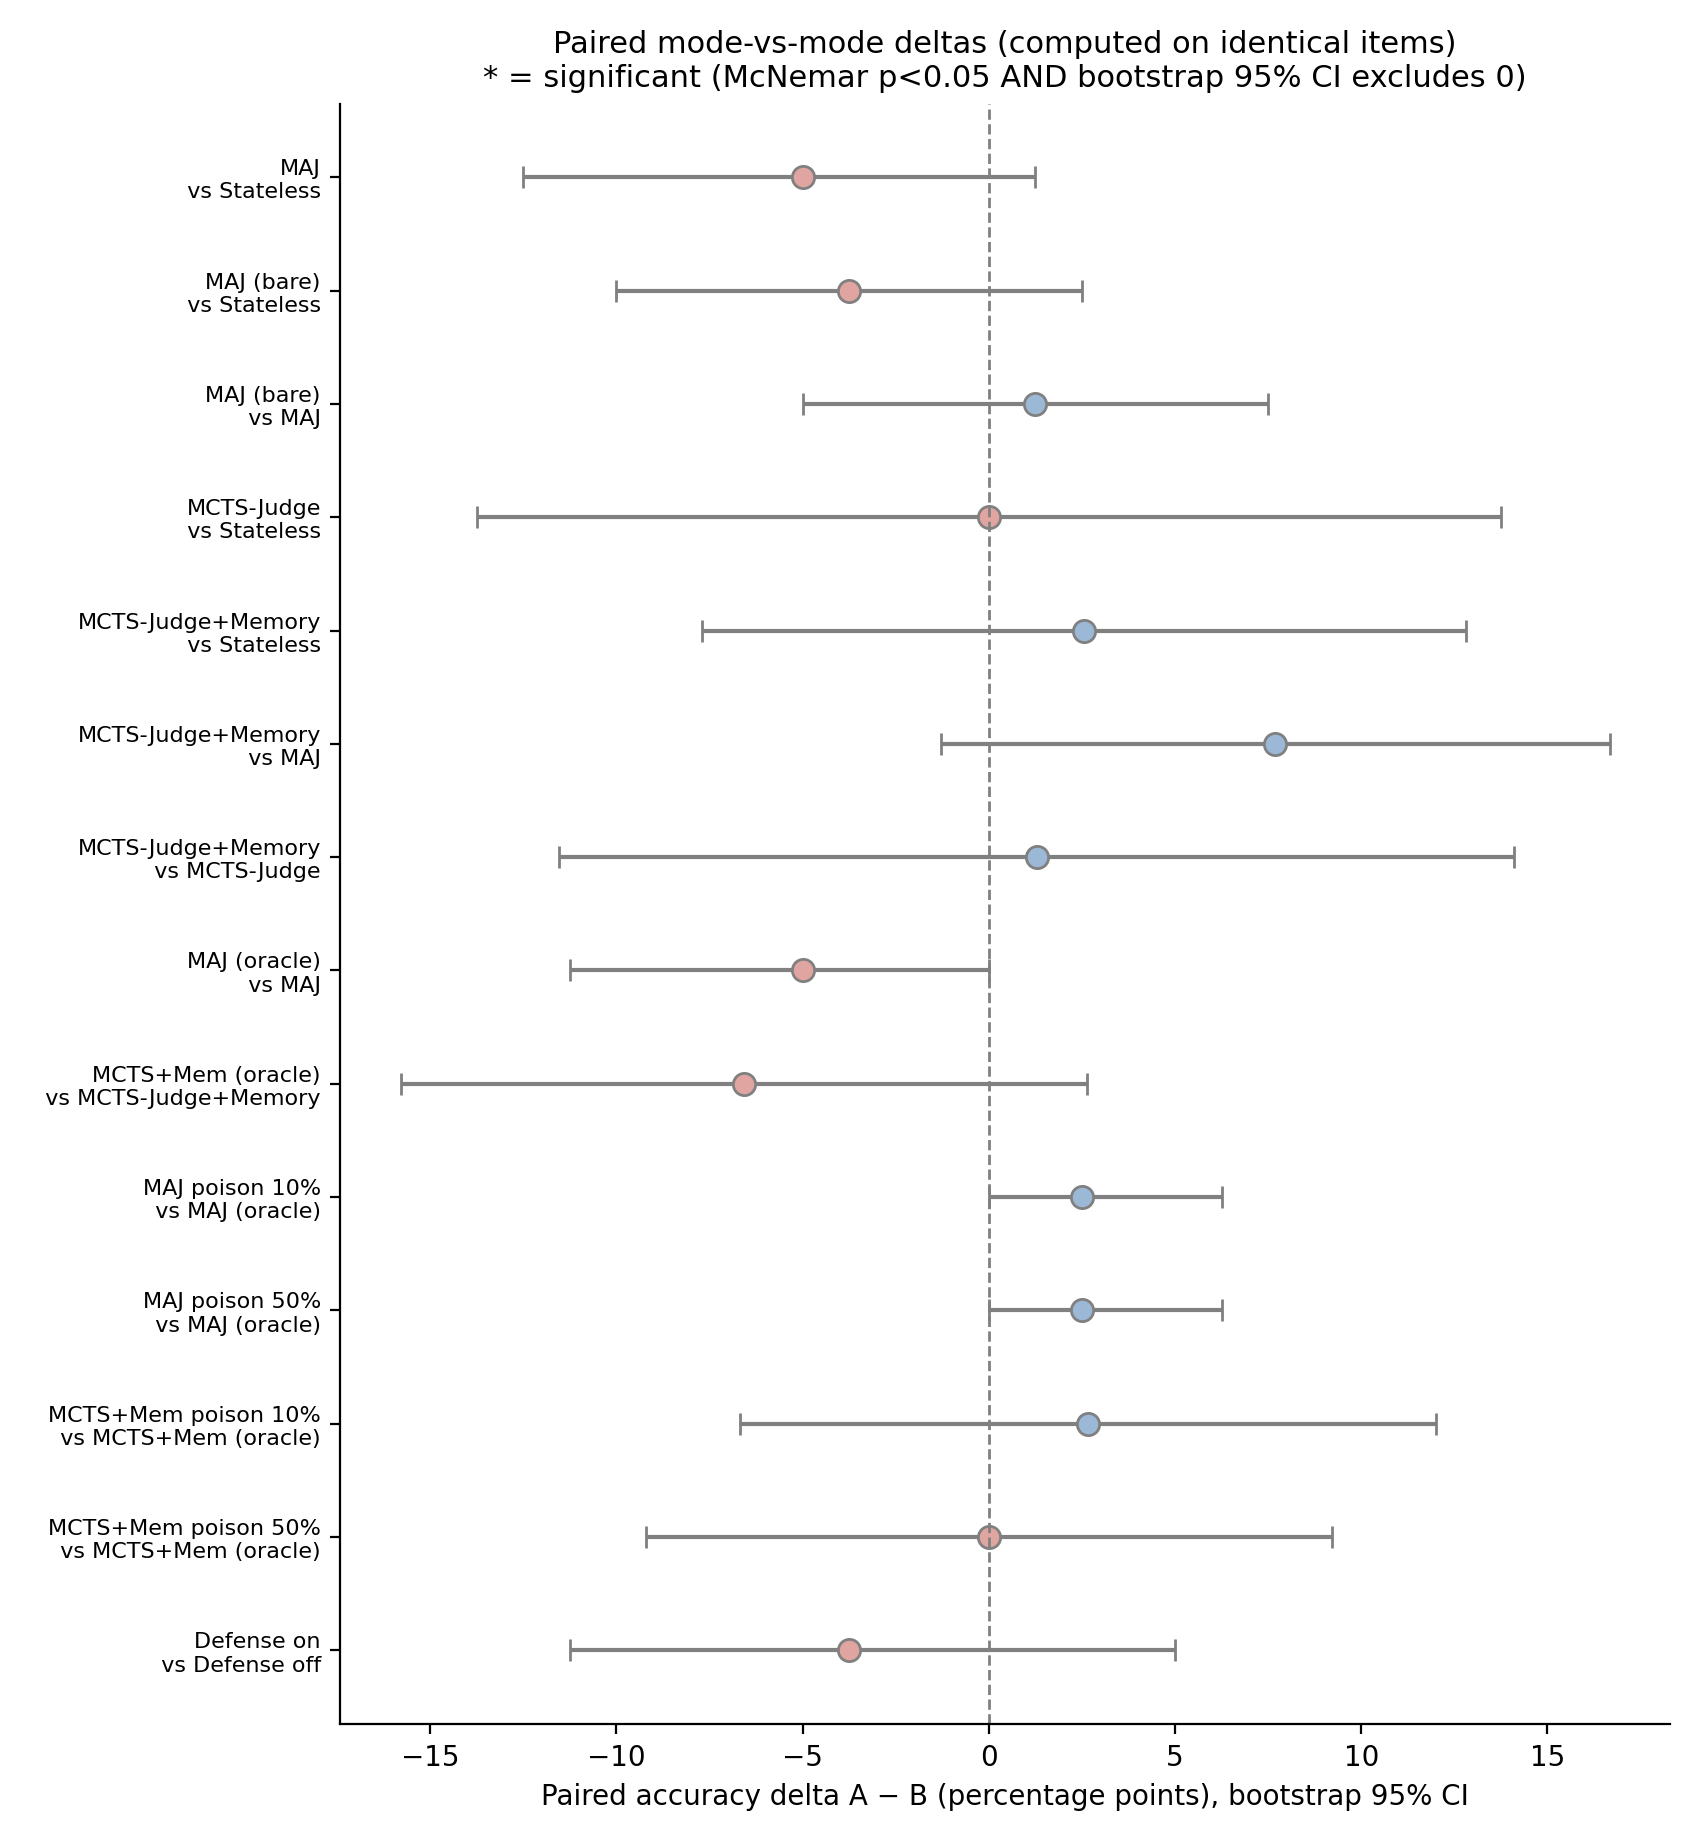
\includegraphics[width=\columnwidth]{figures/paired_deltas.png}
\caption{Paired mode-versus-mode accuracy differences with bootstrap 95\% CIs; every clean-memory interval crosses zero.}
\label{fig:deltas}
\end{figure}

\subsection{Oracle memory, schema ablation, seeds}

We attempted to recover the effect in three ways; none succeeds, and each failure is informative.

\textbf{Provenance.} If the gain is masked by noisy self-written labels, perfectly correct oracle labels should recover it: instead, MAJ drops to 60.0\% ($-5.0$, $p{=}0.22$) and MCTS-Judge+Memory to 65.4\% ($-6.6$, $p{=}0.27$). If the judge were using retrieved labels as evidence, perfect labels should help; they do not. \textbf{Structure.} If the typed schema carries the signal, removing it should hurt: instead, a bare memory with only Policy and Attempt nodes scores 66.2\% [55.4, 75.7], indistinguishable from the full schema (65.0\%) and from stateless (70.0\%) (Figure~\ref{fig:ablation}). The Issue/Fix/Semantic extraction does not earn its complexity here. \textbf{Seeds.} To rule out a split artifact, we re-ran on two further seeds: across seeds 42/123/7, stateless scores 70.0/70.0/67.5 and MAJ 65.0/67.5/66.2; the cross-seed range of a single mode ($\approx$5 points) is wider than any mode-vs-mode gap on a single seed. The small differences we see are sampling noise.

\begin{figure}[t]
\centering
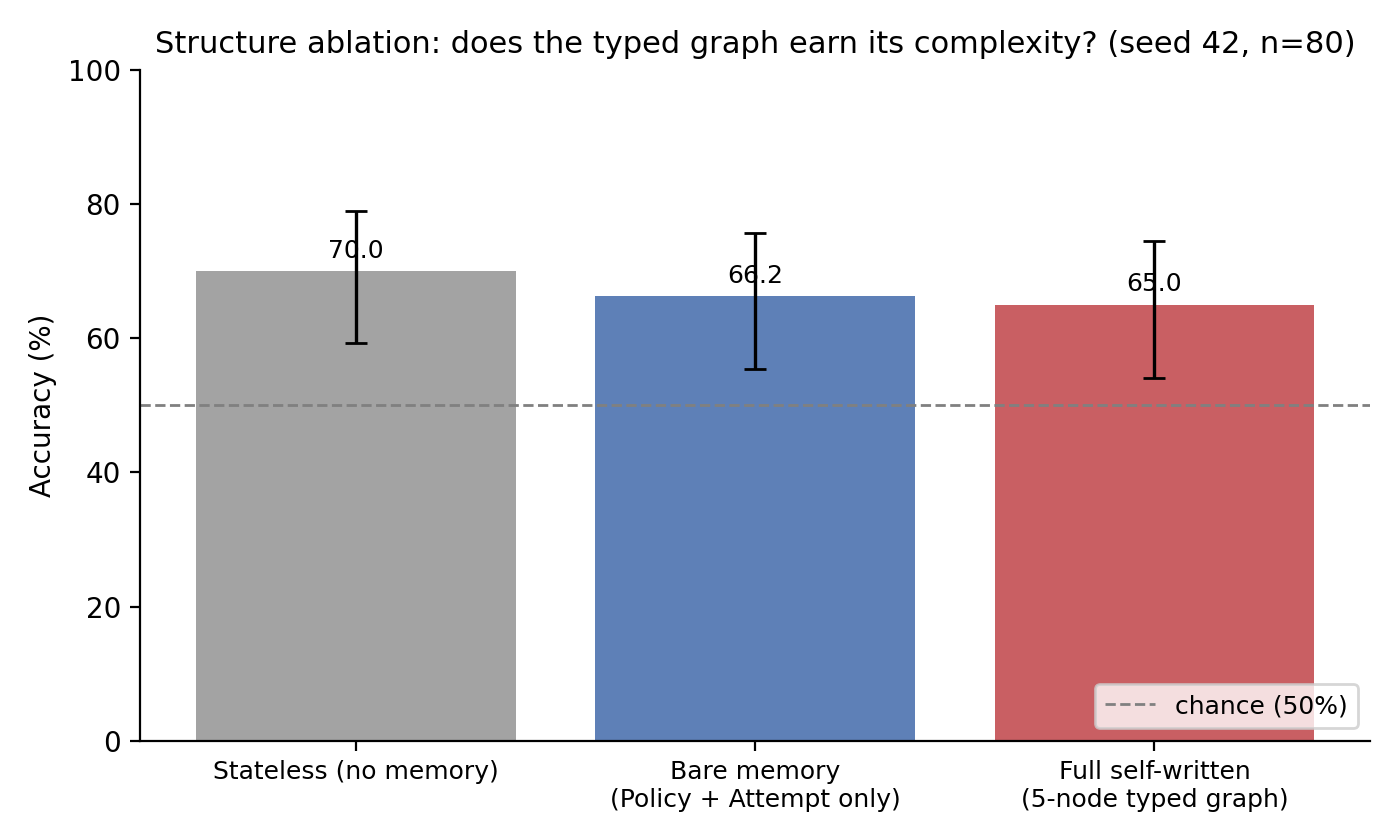
\includegraphics[width=\columnwidth]{figures/structure_ablation.png}
\caption{Structure ablation: stateless baseline, bare Policy-plus-Attempt memory, and the full five-type schema, with Wilson 95\% CIs.}
\label{fig:ablation}
\end{figure}

\subsection{The poisoning artifact}
\label{sec:poisoning}

\begin{table}[t]
\centering
\small
\begin{tabular}{lcc}
\toprule
Poison rate & MAJ & MCTS-J.+Mem. \\
\midrule
0\% (oracle) & 60.0 & 65.4 \\
10\% & 62.5 & 67.5 \\
20\% & 63.7 & 69.7 \\
50\% & 62.5 & 65.4 \\
\bottomrule
\end{tabular}
\caption{Accuracy (\%) under label poisoning, audited harness. Neither mode degrades; for MCTS-Judge+Memory, 50\% vs.\ oracle is a paired $\Delta$ of exactly $0.0$ ($p{=}1.00$).}
\label{tab:poison}
\end{table}

Our earlier, un-audited harness reported that MCTS-Judge+Memory collapsed to 21.2\% at 50\% poisoning, a 49-point drop large enough to serve as a headline finding. Inspection of the per-sample logs showed otherwise: a mid-run network outage had caused a block of samples to error, and the original code scored every errored sample as a wrong answer. With retries and null-verdict exclusion, the same condition scores 65.4\%, identical to oracle (Table~\ref{tab:poison}, Figure~\ref{fig:poison}). The ``poisoning collapse'' was a property of the harness, not the system. A spurious fragility is the same failure mode as a spurious gain; both originated in the measurement.

\begin{figure}[t]
\centering
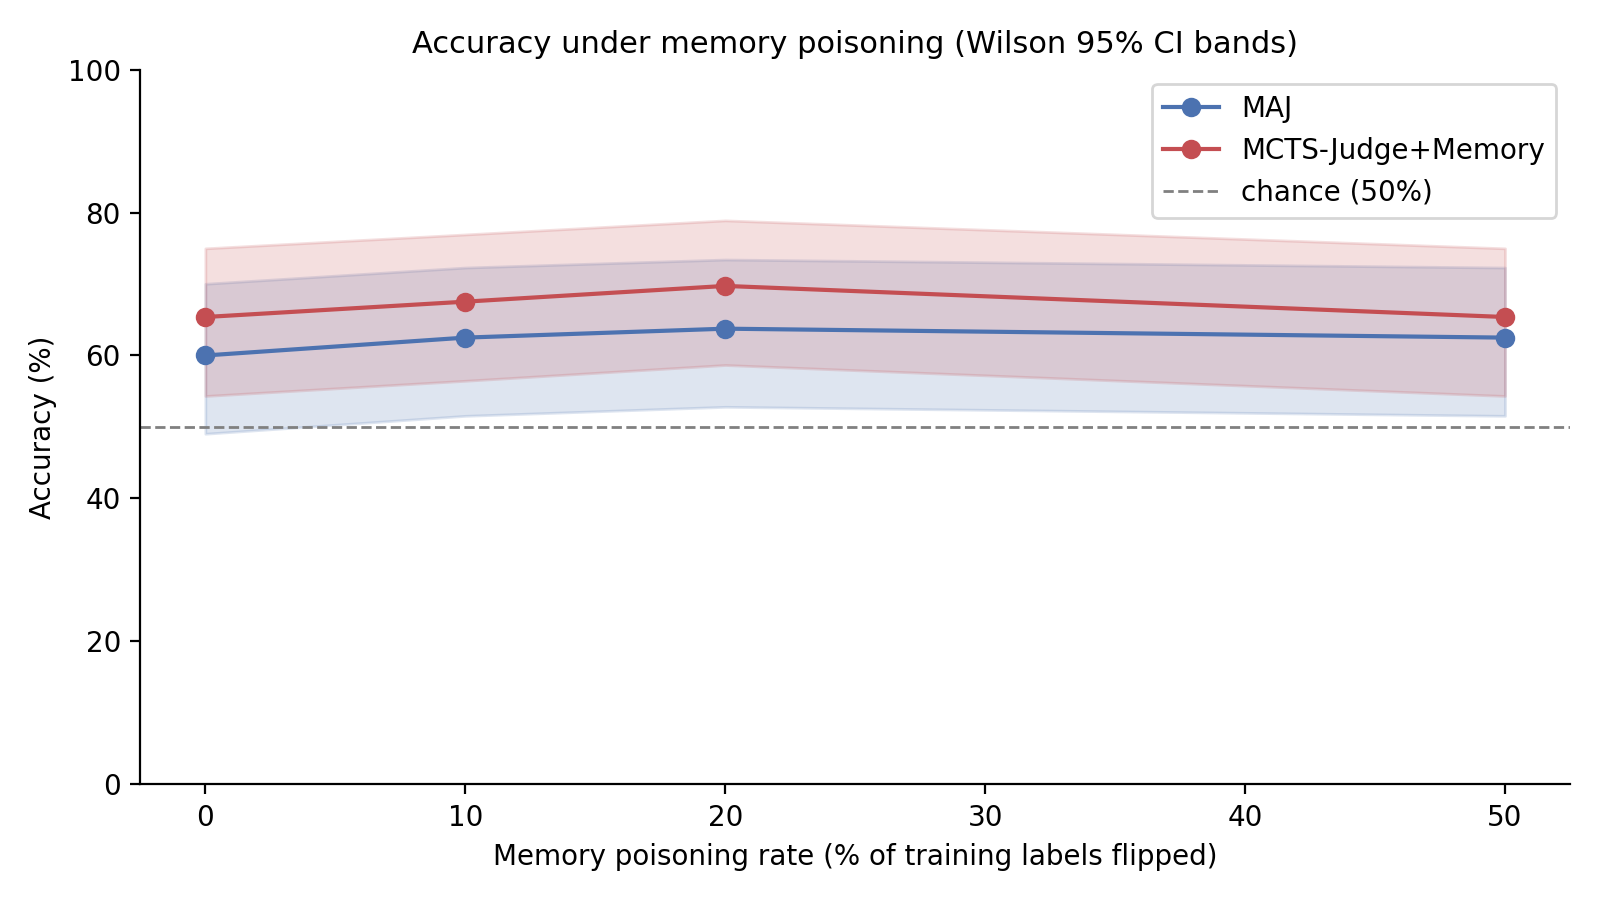
\includegraphics[width=\columnwidth]{figures/poisoning_curve.png}
\caption{Accuracy as a function of the memory poisoning rate under the corrected, audited harness, with Wilson 95\% CI bands; neither mode shows a significant downward trend.}
\label{fig:poison}
\end{figure}

\subsection{Reliability harness}

Accuracy is one number; three more probes say what kind of judge this is. \emph{Stochastic stability}: judge the same item twice and stateless agrees with itself 94\%, MAJ 95\%, MCTS-Judge+Memory 90\%. \emph{Label-flip discrimination}: rewrite a response to invert its ground truth and verdicts flip correctly 65--70\% of the time, similarly across modes. \emph{Defense filter}: a similarity-threshold filter on retrieval under 50\%-poisoned memory does not help (65.0\% vs.\ 64.8\%), an honest negative for that defense. The stability numbers matter below: a judge that already agrees with itself 90--95\% of the time leaves memory very little noise to correct.

\section{Analysis: Why Memory Neither Helped nor Harmed}
\label{sec:analysis}

A null result is only useful if it is explained: what did memory actually do to individual verdicts, why is that the expected behavior, and what design change would escape it?

\subsection{Verdict-flip decomposition}
\label{sec:flips}

\begin{table}[t]
\centering
\small
\begin{tabular}{lcccc}
\toprule
Pair (A vs.\ B) & agree & $b$ & $c$ & $\to$pass \\
\midrule
Stateless / MAJ & 90.0\% & 2 & 6 & 6/8 \\
Stateless / MCTS-J.+M. & 79.5\% & 9 & 7 & 6/16 \\
MAJ self / MAJ oracle & 92.5\% & 1 & 5 & 5/6 \\
MAJ full / MAJ bare & 91.2\% & 4 & 3 & 3/7 \\
\bottomrule
\end{tabular}
\caption{Paired verdict-flip decomposition on identical items ($n{=}80$; $n{=}78$ for the MCTS comparison, whose two null-verdict items are excluded). \emph{agree}: identical verdicts; $b$: items B fixes (A wrong, B right); $c$: items B breaks; $\to$pass: fraction of all changed verdicts that moved toward ``pass''.}
\label{tab:flips}
\end{table}

Every mode judged the identical items, so the effect of memory can be read item by item (Table~\ref{tab:flips}). Three facts emerge.

\textbf{(1) Memory is mostly inert.} MAJ agrees with the stateless verdict on 90\% of items. Swapping self-written memory for oracle changes 7.5\% of verdicts. Deleting three of the five node types changes 8.8\%. The retrieved context block occupies roughly half the prompt and moves almost nothing; the verdict is dominated by the judge's own reading of the task, rubric, and response.

\textbf{(2) The verdicts memory does move follow the judge's bias, not the truth.} For MAJ vs.\ stateless, all six harmful flips turned a correct ``fail'' into a wrong ``pass,'' both helpful flips went the other way, and six of eight flips moved toward ``pass.'' The class-conditional numbers sharpen the picture: every mode is far better on passing items than failing ones (stateless 97.5\% vs.\ 42.5\%), and attaching memory makes the asymmetry \emph{worse} (MAJ: 97.5\% vs.\ 32.5\%). Oracle memory shows the same signature (five of six flips toward pass). Memory here is a leniency anchor: retrieved passing exemplars prime the judge toward ``pass'' on exactly the hard failing items where it was already weakest. The proximate cause is identifiable: the asymmetric retrieval thresholds of \S\ref{sec:system} (positive $\ge 0.85$, negative $\ge 0.92$) systematically admit more passing than failing exemplars into the context, a seemingly innocuous hyperparameter choice that biases the retrieved context by construction.

\textbf{(3) Structured reasoning partially de-anchors.} MCTS-Judge+Memory is the only memory mode whose flips are net-positive ($b{=}9$ vs.\ $c{=}7$), and it shifts the class balance the other way (94.9\% pass / 48.7\% fail): eight of its nine fixes converted false passes into correct fails. Forcing the judge to score 5--7 rubric-specific subtasks before aggregating dampens the holistic leniency prior, consistent with the anchoring account, though the net effect remains insignificant.

\subsection{What memory can contribute, in principle}
\label{sec:theory}

Let $X$ be the stateless input (task, rubric, response), $Y \in \{\text{pass},\text{fail}\}$ the label, and $M$ the retrieved memory. The quantity of interest is the accuracy of the \emph{Bayes-optimal} decision rule, which for any available conditioning information $Z$ predicts $\arg\max_y P(Y{=}y \mid Z)$ and attains accuracy $A^*(Z) = \mathbb{E}_Z\!\left[\max_y P(Y{=}y \mid Z)\right]$. Comparing the stateless conditioning $X$ to the memory-augmented conditioning $(X,M)$:

\begin{proposition}[Bayes ceiling]
\label{prop:bayes}
$A^*(X,M) \ge A^*(X)$ always, and the gain is governed entirely by how much the posterior moves when $M$ is revealed:
\[
A^*(X,M) - A^*(X) \;=\; \mathbb{E}_{X,M}\!\big[\max_y P(Y{=}y\mid X,M)\big] - \mathbb{E}_{X}\!\big[\max_y P(Y{=}y\mid X)\big],
\]
which is zero whenever $P(Y\mid X,M)=P(Y\mid X)$ for almost all $(X,M)$, in particular whenever $Y \perp M \mid X$. Conversely the gain is strictly positive only on the event that revealing $M$ flips which class is most probable.
\end{proposition}

In words: memory can raise the achievable accuracy only to the extent that the conditional label distribution given $(X,M)$ actually differs from the one given $X$ alone; if memory is conditionally uninformative about the label, the Bayes-optimal accuracy is unchanged regardless of the decision rule. This is the claim our protocol is designed around, and it does \emph{not} require a mutual-information argument: it follows directly from the definition of $A^*$ and the fact that $\max_y P(Y{=}y\mid X,M)$ is a $\sigma(X,M)$-measurable refinement of $\max_y P(Y{=}y\mid X)$.

\emph{Is $M$ conditionally informative here?} The protocol is built to make $P(Y\mid X,M)\approx P(Y\mid X)$: the question-level split guarantees no retrieved item concerns the test question, the rubric is fully specified inside $X$, and graded financial QA sits within GPT-4o's parametric competence, so a neighboring question's verdict shifts the posterior negligibly. The oracle experiment is the empirical test: if revealing perfectly correct retrieved labels moved the posterior, oracle memory would raise accuracy; instead it is worth nothing ($-5.0$ and $-6.6$ points, n.s.), which is what Proposition~\ref{prop:bayes} predicts when $M$ carries no conditional signal and is difficult to explain otherwise.

\emph{A separate, smaller channel: realized-judge noise.} The proposition bounds the \emph{Bayes-optimal} accuracy. The judge we actually deploy is a stochastic rule $f$, not the Bayes rule, so conditioning on $M$ could in principle also help by stabilizing $f$ toward its own posterior even when $A^*$ is unchanged. We do not claim memory cannot help through this route; we report only that the room for it is small here. The stability probes (\S\ref{sec:flips} context) show the judge disagrees with itself on just 5--10\% of items, so the realized judge already sits close to a deterministic rule, and any stabilizer, memory or otherwise, has at most that 5--10\% of verdicts to move. Self-disagreement is thus a \emph{diagnostic} for how much stochastic instability exists to be corrected, not a bound on all conceivable benefit of memory.

This decomposes the realized accuracy change into the rate at which memory changes a verdict and the quality of those changes:
\[
\mathbb{E}[\Delta] \;=\; \underbrace{P(\text{flip})}_{0.10 \text{ for MAJ}} \cdot \bigl(2q - 1\bigr), \quad q = P(\text{flip corrective}),
\]
and the decomposition in \S\ref{sec:flips} measures $q = 2/8$ for MAJ. When $M$ does not move the posterior (\S\ref{sec:theory}), the flips that do occur are driven by the stylistic content of $M$ (here, the exemplar imbalance) rather than by label evidence, so $q$ falls below $1/2$ and memory mildly hurts, in the direction of the judge's prior bias. Substituting the measured values gives $0.10 \times (2 \cdot 0.25 - 1) = -5.0$ points, matching the observed MAJ delta. The same expression explains the conventional-protocol illusion: leakage makes $P(Y\mid X,M)$ depend sharply on $M$ (the paired item's verdict is now in memory), pushes $q$ far above $1/2$, and manufactures the 6--10 point ``gain.''

\subsection{Practical remedies, and when memory should help}
\label{sec:remedies}

The account above is constructive; it identifies exactly which levers exist.

\paragraph{(a) Balance the contrastive signal.} The leniency tilt is a property of the retrieval design, not of memory per se. Symmetric thresholds, or enforcing equal numbers of passing and failing exemplars in the context block, remove the systematic push toward ``pass'' that produced MAJ's $-5.0$. This is a minimal, directly testable change.

\paragraph{(b) Gate memory by informativeness.} $\mathbb{E}[\Delta]$ is negative whenever $q<1/2$, so memory should be injected only when retrieval is likely to be evidential, e.g.\ when the top retrieved attempt is a near-duplicate of the current item, falling back to the stateless judge otherwise. Gating bounds the harm at zero by construction and preserves the benefit on recurring items, the one regime where $P(Y\mid X,M)$ genuinely departs from $P(Y\mid X)$.

\paragraph{(c) Use memory at the population level.} The judge's dominant failure is a stable class bias (42.5\% on failing items), and a store of past evaluations is exactly the data needed to \emph{measure} that bias per Semantic category. Instead of injecting instance-level exemplars, let memory supply a calibration correction: a per-category decision-threshold shift estimated from stored (verdict, outcome) pairs. This converts the graph from an ineffective evidence channel into a statistically well-grounded bias-correction channel, and it is the use we consider most promising.

\paragraph{(d) Target regimes where memory moves the posterior.} Proposition~\ref{prop:bayes} predicts memory helps when the judge cannot already solve the task from $X$: weaker judge models with headroom below the rubric; domains whose verdicts depend on conventions the model has never seen (project-specific style guides, private grading norms); workloads with recurring or near-duplicate items. These are falsifiable predictions. They also mark the boundary of our claim: the result is ``no effect for GPT-4o on this benchmark,'' not ``memory never helps,'' and our data do not support the latter.

\section{Conclusion}

We asked when persistent memory helps an LLM judge, and we required an answer whose measurement could be proven sound. The protocol (question-level partition, frozen memory, a two-layer cryptographic audit) proves the absence of memory leakage per run, and it caught a real leakage defect in our own code on its first application. Under this protocol the answer, for GPT-4o on this benchmark, is that no benefit is measurable: neither memory nor tree search outperforms the stateless judge, and an apparent 6--10 point gain and an apparent poisoning collapse were both artifacts of the measurement. The per-item analysis explains why: under the leakage-free protocol the conditional label distribution barely moves when memory is revealed, so the Bayes-achievable gain is near zero, while the separate route of stabilizing the stochastic judge has only its 5--10\% self-disagreement to exploit; the few verdicts memory does change follow the judge's leniency bias, traceable to an asymmetric retrieval setting with a minimal fix. The general lesson is that both the promise and the fragility of judge memory, as commonly measured, are properties of the harness: trustworthy claims about memory-augmented judging require audited measurement first. We release the protocol, audit, per-sample records, and a one-command reproduction script so the practice can be adopted directly.

\section*{Limitations}

\textbf{Power.} $n{=}80$ gives a minimum detectable effect of roughly 12--15 points: sufficient to test the conventional protocol's 6--10 point claim, which it refutes, but not to exclude a genuine effect of a few points. We therefore state the result as ``no effect detected at this scale.'' \textbf{Single judge, single benchmark.} All audited results use GPT-4o on graded financial QA; \S\ref{sec:remedies}(d) states explicitly where we expect the picture to change. \textbf{Excluded samples.} At most four samples per configuration errored after retries and were excluded; scoring every one of them as incorrect changes no significance conclusion. \textbf{Poisoning pattern.} We tested uniform random label flips only; structured adversarial poisoning may behave differently. \textbf{Conventional-protocol numbers.} Their per-sample logs were not retained, so they are reported as a motivating observation, not a verified claim. \textbf{Audit scope.} The audit proves the absence of the two channels we model (graph mutation during evaluation, paired-item splitting); it does not address side channels outside the memory store.

\section*{Acknowledgments}
This work was carried out at Innopolis University. We thank the EvalsBench authors for the open benchmark.

\bibliography{references}

\appendix

\section{Complete Audited Results}
\label{app:full}

\begin{table}[h]
\centering
\small
\begin{tabular}{lcc}
\toprule
Configuration & Acc.\ [95\% CI] & $n$ \\
\midrule
Stateless & 70.0 [59.2, 78.9] & 80 \\
MAJ, self-written & 65.0 [54.1, 74.5] & 80 \\
MAJ, oracle & 60.0 [49.0, 70.0] & 80 \\
MAJ, poison 10\% & 62.5 [51.5, 72.3] & 80 \\
MAJ, poison 20\% & 63.7 [52.8, 73.4] & 80 \\
MAJ, poison 50\% & 62.5 [51.5, 72.3] & 80 \\
MAJ, bare schema & 66.2 [55.4, 75.7] & 80 \\
MCTS-Judge, no memory & 70.0 [59.2, 78.9] & 80 \\
MCTS-J.+M., self-written & 71.8 [61.0, 80.6] & 78 \\
MCTS-J.+M., oracle & 65.4 [54.3, 75.0] & 78 \\
MCTS-J.+M., poison 10\% & 67.5 [56.5, 76.9] & 77 \\
MCTS-J.+M., poison 20\% & 69.7 [58.7, 78.9] & 76 \\
MCTS-J.+M., poison 50\% & 65.4 [54.3, 75.0] & 78 \\
\bottomrule
\end{tabular}
\caption{All audited configurations (GPT-4o, seed 42). Where $n<80$, the remaining samples errored after retries and were excluded with null verdicts.}
\label{tab:appfull}
\end{table}

\section{Class-Conditional Accuracy}
\label{app:class}

\begin{table}[h]
\centering
\small
\begin{tabular}{lcc}
\toprule
Mode & Pass items & Fail items \\
\midrule
Stateless & 97.5 & 42.5 \\
MAJ (self-written) & 97.5 & 32.5 \\
MCTS-Judge + Memory & 94.9 & 48.7 \\
\bottomrule
\end{tabular}
\caption{Accuracy (\%) by ground-truth class ($n{=}40$ per class; $n{=}39$ for MCTS-Judge+Memory, whose null-verdict items are excluded). All modes share a pass-oriented bias; instance-level memory amplifies it, subtask decomposition dampens it.}
\label{tab:appclass}
\end{table}

\section{Audit Record Format}
Each run emits a machine-readable record holding the before/after snapshots (per-type node and relationship counts, total counts, SHA-256 fingerprint over sorted node identifiers and edge triples) and their diff. A run is leakage-free only if the diff is empty and the fingerprints match; records are released with the code.

\end{document}
